\chapter{Existing Approaches in Behavior Analysis and Detection of Customer Satisfaction}
\label{ch:backgroundResearch}
As the cornerstones of the research objectives have been defined, the goal is to shed more light onto the key point this thesis deals with, namely Customer Satisfaction. The following chapter defines the term Customer Satisfaction and outlines which properties are paid attention to in this thesis. Moreover, existing approaches related to analysis of usage behavior and measurement of Customer Satisfaction, with focus on their relevance regarding this thesis, will be discussed in more detail.

\section{Definition and Limitations of Customer Satisfaction}
\label{sec:custSatisfactionDefinition}
Before evaluating approaches to determine Customer Satisfaction via collected knowledge data, the term should be properly understood. Research papers regarding the definition of Customer Satisfaction were already published in the 70s. Since then different approaches viewing the topic from slightly different angles have been proposed. A popular statement, namely that Customer Satisfaction is based on the comparison between individual expectations of the customer and the perceived performance of the product after usage was the common result of research experiments at these times \cite{oliver1977effect} \cite{anderson1973consumer}. If his or her expectations were lower or equal, the customer can be considered as satisfied whereas vice versa the customer is dissatisfied since his expectations were not fulfilled. In case the expectations do not match with the actual performance of the product this is also named positive- respectively negative disconfirmation while a match is described as confirmation \cite{oliver1977effect} \cite{anderson1973consumer}.

As a result, when imagining it in a more mathematical way Customer Satisfaction can be represented as a simple function with two input parameters. One the one hand, the expectations of the customer are based on all information gathered before using the product. It is an subjectively built ideal picture of the product depending on advertisement, word-of-mouth critics and company- respectively brand reputation \cite{johnson2001evolution} \cite{neckel2015}. On the other hand the perceived performance of the product when using it comprises the whole consumption experience of the customer. As the main driver of this experience, the overall provided quality of the product was identified. This perceived quality metric not only covers the pure quality, in terms or whether the product reliably performs as advertised, but more exactly specifies the actual quality for the price. Thus, when talking about drivers of Customer Satisfaction it is often described as perceived value \cite{johnson2001evolution} \cite{fornell1992national}. Along with the shift towards importance of customer retention, Customer Satisfaction models developed from a transaction tied view to a cumulative view which considers a customers experience with a product over a longer time period. This view more specifically includes the fact that customer expectations change over time and become influential for the perceived quality as well. \cite{johnson1996expectations}. It became clear that the Customer Satisfaction construct is quite involved and especially some of the antecedents and consequences remained unclear. 

The Swedish Customer Satisfaction Barometer (SCSB) was a big research project in investigating Customer Satisfaction across several industries within a whole country. It used a model based on the two identified input parameters from previous research. The positive result of Customer Satisfaction was already anticipated by \cite{bolton1998dynamic} \cite{gustafsson2005effects}. The outcome of dissatisfaction was based on the theory of \cite{hulett1971exit} that customers are more likely to complain for problems they might have. Furthermore the model stated that positive resolving of complaints supports the establishment of loyalty against the company. A sketch of this model is shown in figure \ref{fig:scsb}

\begin{figure}
	\centering
	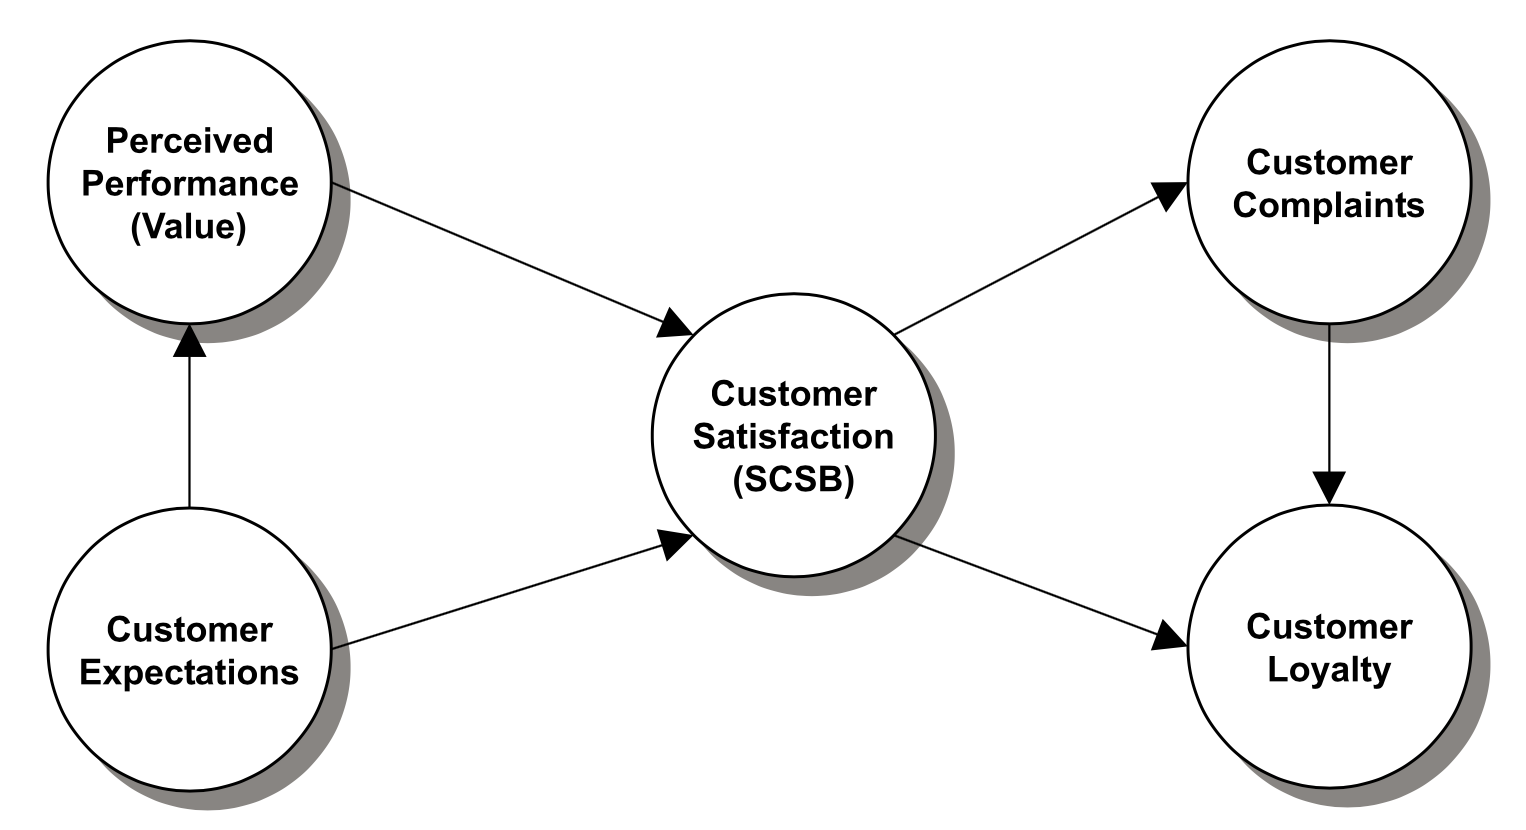
\includegraphics[width=1.0\textwidth]{img/scsb.png}
	\caption{Model used for Swedish Customer Satisfaction barometer \cite{fornell1992national}}
	\label{fig:scsb}
\end{figure} 

Although the model experienced some critics in the following years as further national Customer Satisfaction surveys were deployed they all were based on and inspired by the original ideas of the swedish model. A more enhanced analysis of the existing model approaches was done by \cite{johnson2001evolution}. As a result of the derived strengths and weaknesses from different Customer Satisfaction barometer models, they proposed a new model which will be used as the base model by this thesis to build its further empirical work on. The model is visualized in figure \ref{fig:satisfactionModel}. Each of the different parts will be described briefly to get an overview on the essential components and their relationships, adaptations in contrast to the initial base model, namely the SCSB, and the limitations drawn by the author regarding the work in this thesis. 

\begin{figure}
	\centering
	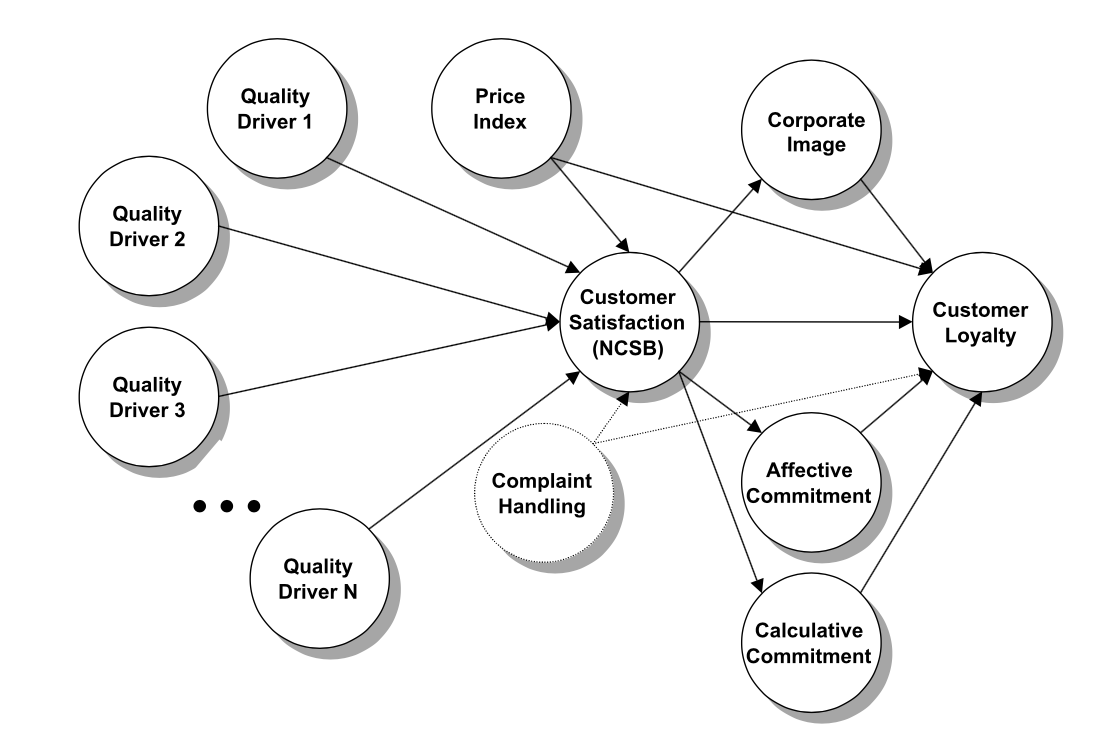
\includegraphics[width=1.0\textwidth]{img/custSatisfaction.png}
	\caption{Customer satisfaction model proposed by \cite{johnson2001evolution}}
	\label{fig:satisfactionModel}
\end{figure} 

The first difference when comparing the latter proposed model with the SCSB is the role of customer expectations. Since satisfaction has to be observed within a long time period, expectations get adapted throughout repeated consumption experience as well. More emphasis is put on the quality delivered by the product and the expectations are considered to be evaluated regularly due this quality. These statements can be supported among several industries including the communications sector which the author considers as similar to the sector the case study of this thesis operates in \cite{johnson1996expectations} \cite{fornell1996american}. Despite that fact the author does not completely agree with these findings to remove the term "customer expectations" totally. Instead of the expectation parameter, 1-n perceived quality criterion are predictors for Customer Satisfaction. Next to the quality drivers the perceived price for the provided product quality plays a role as well. The third satisfaction driver illustrated in this model are complaint handling. Due to evolvement of customer support services, customer complaints cannot be stated as simple negative outcome of Customer Satisfaction. More specifically customer care influences emotions either negatively or positively and as a consequence is in direct predictor relationship to satisfaction. It may even have an impact on repurchase behavior of customers which explains the direct relationship to customer loyalty \cite{johnson2001evolution}. 

The three remaining components have not yet been mentioned explicitly regarding their role in the customer satisfaction construct. All of them are directly influenced by the outcome of Customer Satisfaction while mediating the loyalty parameter. The corporate image, or sometimes called brand reputation, indicates how popular and known company is in the public. Consumption experiences of a customer affects the corporate image in a certain direction as well. According to a study of \cite{hussain2015service} a dissatisfied customer tells on average nine other people about negative experiences which can heavily affect loyalty. Although the corporate image is part of the model it will not be discussed or used further in the empirical work of this thesis because it can not be measured by usage behavior and quality data. Similarly the affective- and calculative commitment mediate parts of the effect of Customer Satisfaction on customer loyalty. While the affective component resides on the emotional side and mainly relates to trust with regard to a brand, the calculative component is more rational in terms of costs. (e.g.: costs for a customer to cancel a relationship and switcht to a competitor) \cite{johnson2001evolution} Both components were mentioned for the purpose of completness but are not elaborated in more detail since they cannot be represented in the available data of the case study. 

\section{Measurement of Customer Satisfaction}
As the reader got an overview on the parts and influential factors of Customer Satisfaction, the next step is to look at possibilities to transform the defined model properties to quantitative measurements. On the one hand this thesis evaluated survey based measurements and looked in more detail on different types and their performance. On the other hand it was tried to find approaches to measure Customer Satisfaction without survey data based on implicit satisfaction representing patterns in huge data sets. 

\subsection{Theories about Customer Satisfaction determination}
Although there has been a lot of research regarding a formal definition of Customer Satisfaction, less papers were published on how this satisfaction can be quantitatively measured. One approach based on the original expectancy-performance disconfirmation model was to design a survey asking customers how they would rate

\begin{itemize}
	\item their expectations regarding to a set of chosen dimensions before usage and
	\item the perceived performance and quality of the product with regard to the same set of product dimensions \cite{prakash1983reliability}.
\end{itemize}

This approach seems to be promising as it respects the originally identified and well researched Customer Satisfaction model. However, it brings problems regarding the expectation parameter with it and thus make it inappropriate for this thesis. Firstly, expectations can hardly be measured unbiased since they get evaluated by the customer alongside with the perceived quality in case of using one satisfaction survey \cite{getty1995relationship}. As outlined in \ref{custSatisfactionDefinition} the proposed model is based on cumulative satisfaction evaluation which yields regular adaptations on what a customer expect from a product. Asking customers about their expectations, with regard to a specific set of product dimensions, explicitly before usage neither makes any sense from a business perspective of Tractive nor is the author able to initiate a process to collect such data. Secondly, measuring customer expectations turns out to be difficult as people tend to rate their expectations, if they have to state them explicitly, very high on average \cite{babakus1992empirical}. As a consequence the uniform overrating of customers expectations will not provide any extra information in assessing customer satisfaction from a survey. As last point in the considerations of the author regarding this approach, the validity of stated expectations has to be questioned since customers often do not have specific expectations before using a product. A dominant reason for this phenomenon is especially observed in software products or services due to its variable and intangible nature. Following, it was found that if customer expectations cannot be formed well, the expectancy-performance disconfirmation metric looses its worth \cite{halstead1994multisource}. 

The mentioned arguments and following impracticality required the need for further research on suitable approaches to assess Customer Satisfaction. In contrast to the research branch which insists on the importance of considering expectations in measurement, there has also been research experience in favoring the perceived performance or, depending on the Customer Satisfaction model, the perceived value \cite{yuksel1998customer}. Based on the mentioned disadvantages in assessing expectations it is claimed that perceived performance reflects the subjective response and emotional feeling as outcome of a consumption experience and thus is seen as the major source in steering the satisfaction value into a particular direction \cite{halstead1994multisource} \cite{cronin1992measuring}. Although perceived performance alone is claimed to perform well as measurement indicator for Customer Satisfaction, a lot of different data dimensions tie together an overall quality or performance. Depending on the dataset the collected parts can correlate in a certain way, be independent, redundant or differ by their importance in contributing to the overall satisfaction. Thus, taking the importance of quality indicators into account can be crucial in determining why a customer might be more satisfied than a similar one \cite{barsky1992customer}. Based on these findings and results in past research this thesis follows, with regard to the case study, the hypothesis that collected usage behavior data is especially of interest if related to quality and performance of the product respectively offered service. With a view to the upcoming empirical work, the available data at Tractive provides enough quality and performance indicators. This data is collected transactional-oriented with the customers usage of the Tractive GPS products and can be used when following the path of this measurement approach. 

\subsection{Quantitative metrics for classification of satisfaction outcome}
Before being able to elaborate on the taxonomy of statistical- and data-mining related methods, the open question, on how a Customers satisfaction feeling can be measured reliably by quantitative metrics, has to be answered. 

In order to be able to reveal reliable patterns and influencing factors in quality and performance data when executing analysis methods, some sample satisfaction data from customers is needed. Otherwise no educated comparisons of results are possible and the results would only be wild guesses. Due to the complexity of building a customers attitude towards a product, the preferred way is to collect quantitative data representing satisfaction by a survey \cite{yuksel1998customer} \cite{hayes1998measuring}. Especially the software industry is a sector where it is hard to classify a customers satisfaction based on objective data implicitly gathered by the systems without asking any person \cite{hayes1998measuring}. However, conducting a Customer Satisfaction survey turns to be a difficult task. On the one hand it should support later analysis by enough sample data, while on the other hand it should also collect enough useful satisfaction measurements from customers to derive expressive results \cite{sauermann2013increasing}. 

There have been different opinions in research on how a Customer Satisfaction survey should be structured and how comprehensive the content should be. \cite{hayes1998measuring} proposed a process where all quality dimensions of a product, considered as important by the survey issuer, should be collected since this promises to provide a complete view on the whole product separated by its characteristics. The author of this thesis sees this differently because the research objective is to reason about an overall satisfaction of customers without knowing any subjective opinion from them. Plus, response rates will decrease the more items a survey contains and the essential priorities for the researcher is first, collecting many survey answers to have a bigger chance in finding significant patterns and learn more reliably from the data and second, keeping understandability of results rather simple \cite{sauermann2013increasing}. In dependence on the scarce resources of businesses in very competitive markets, as the software industry for instance, approaches and outcomes of research developed into the direction of making surveys much shorter but with wisely chosen questions which are useful to reason about loyalty of customers which in turn is strongly connected to profit \cite{reichheld2003one}. When designing a Customer Satisfaction survey to collect sample data for the analysis part these latter ideas were taken under consideration. 

\section{Taxonomy of methods for behavioral analysis and satisfaction prediction}
